%!TEX root = ../thesis.tex

\subsection{提案モデルの識別可能性}

本節では、前節で定義したDAGモデルの識別可能性を証明する。
提案モデルは、連続変数と離散変数とが混在することを許容するDAGモデルであるため、
その特殊形として、全てが連続変数であるモデルや全てが離散変数であるモデルを考えることも可能である。
全てが連続変数である場合は、Additive Noise Modelとなり、
モデルの識別可能条件が複数証明されている\cite{Shimizu2006-yu}
\cite{Hoyer2008-oo}
\cite{Peters2013-eb}
\cite{Peters2014-ro}
\cite{Park2020-ey}。
また、全てが離散変数である場合は、QVF-DAGモデル\cite{Park2017-hw}となり、
識別可能性が既に証明されている\cite{Park2017-hw}。
そこで以下では、観測変数集合に連続変数と離散変数の両方が含まれる場合に関する識別可能条件について議論する。
まず、証明の方針について直感的な理解を得るために、
図\ref{fig:prop_three_variate}のような3変数モデルを用いてその識別可能性を示す。
ここで$X,Z$は連続変数、$Y$は離散変数であるとする。
図\ref{fig:prop_three_variate}の3つの因果グラフから生成される分布は、
いずれも$X \indep Z | Y$という条件付き独立関係が成立しており、
因果マルコフ条件のみでは識別できない例である。
しかし、以下で示すように、提案モデルの特徴を利用すると識別することが可能である。

\begin{align*}
  G_1 \colon & X = \theta_{X} + e_X, \quad e_X \sim N(0, \sigma_X^2) \\
             & Y|X \sim \mathit{Poisson}(\lambda), \quad \log(\lambda) = \theta_Y + \theta_{YX}X \\
             & Z = \theta_Z + \theta_{ZY}Y + e_Z, \quad e_Z \sim N(0, \sigma_Z^2)
\end{align*}

\begin{align*}
  G_2 \colon & X = \theta_X + \theta_{XY}Y + e_X, \quad e_X \sim N(0, \sigma_X^2) \\
             & Y|Z \sim \mathit{Possion}(\lambda), \quad \log(\lambda) = \theta_Y + \theta_{YZ}Z \\
             & Z = \theta_{Z} + e_Z, \quad e_Z \sim N(0, \sigma_Z^2)
\end{align*}

\begin{align*}
  G_3 \colon & X = \theta_X + \theta_{XY}Y + e_X, \quad e_X \sim N(0, \sigma_X^2) \\
             & Y \sim \mathit{Poisson}(\lambda) \\
             & Z = \theta_{Z} + e_Z, \quad e_Z \sim N(0, \sigma_Z^2)
\end{align*}

\begin{figure}[ht]
  \centering
  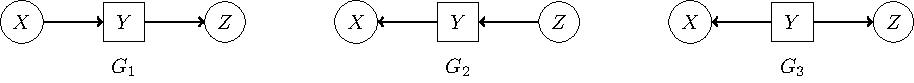
\includegraphics{./picture/prop_three_variate.pdf}
  \caption{3変数のDAGモデル}
  \label{fig:prop_three_variate}
\end{figure}

命題\ref{prop:MRS}より、$G_1, G2$においては
\begin{align*}
  E(Y^2) > E(Y) + E(Y)^2
\end{align*}
である一方で、$G_3$においては
\begin{align*}
  E(Y^2) = E(Y) + E(Y)^2
\end{align*}
となる。
よって、離散変数のモーメント比~\eqref{eq:MRS}が1か1以上かを確かめることで
$G_1, G_2$と$G_3$は識別可能である。

次に$G_1$について、もし連続変数$X, Z$の誤差変数の分散が
$\sigma_X^2 < \sigma_Z^2 + \mathit{Var}(E(Z|Y))$を満たすならば、
全分散の公式を用いて以下が成り立つ。
\begin{align*}
  \mathit{Var}(Z) &= E(\mathit{Var}(Z|Y)) + \mathit{Var}(E(Z|Y)) \\
                  &= \sigma_Z^2 + \mathit{Var}(E(Z|Y)) \\
                  &> \sigma_X^2 \\
                  &= \mathit{Var}(X)
\end{align*}

よって、$X$のほうが因果順序が早いことが分かる。
つまり、誤差変数の分散が$\sigma_X^2 < \sigma_Z^2 + \mathit{Var}(E(Z|Y))$を満たすならば、
因果順序を特定することが可能である。

$G_2$についても同様に、
連続変数$X, Z$の誤差変数の分散が、
$\sigma_Z^2 < \sigma_X^2 + \mathit{Var}(E(X|Y))$を満たすならば、
真の因果順序$\pi = (Z, Y, X)$を特定することが可能である。


ここからは、上記の3変数モデルでの証明の方針を拡張し、
提案モデルが一般的なp変数の場合においても識別可能であることを証明する。

\begin{theo}[提案モデルの識別可能性]
  \label{theo:prop_identifiability}
  定義\ref{prop_model}によって定義されるDAGモデルは、以下の仮定を満たすとき識別可能である。
  ただし、DAG $G$における因果順序を$\pi$で表す。
  \begin{itemize}
    \item
    連続変数が割り当てられた任意の頂点$j = \pi_m \in C, k \in De(j) \subset C$の
    データ生成過程における誤差変数の分散について、以下が満たされている。
    \begin{equation*}
      \sigma_j^2 < \sigma_k^2 + E(\mathit{Var}(E(X_k | X_{Pa(k)}) | X_{\pi_1}, \dots, X_{\pi_{m-1}}))
    \end{equation*}

    \item
    離散変数が割り当てあられた任意の頂点$j \in D$について、
    $\beta_{j1} > -1$が満たされている。
  \end{itemize}
\end{theo}

2点目の仮定は、ベルヌーイ分布や多項分布によるDAGモデルを除外するための仮定である。
なぜななら、ベルヌーイ分布や多項分布によるDAGモデルは識別不能であることが知られているためである\cite{Heckerman1995-es}。

以下では、定理\ref{theo:prop_identifiability}を証明する。

\begin{proof}
  一般性を失わずに、真の因果順序が一意であり、$\pi = (\pi_1, \dots, \pi_p)$であると仮定する。
  また、簡単のために、$X_{1:j} = (X_{\pi_1}, X_{\pi_2}, \dots, X_{\pi_j})$、
  $X_{1:0} = \emptyset$と定義する。
  DAG $G$において、
  連続変数に割り当てられた変数からなる頂点の集合を$C$、
  離散変数に割り当てられた変数からなる頂点の集合を$D$とする。
  加えて、モーメント関連関数$f(\mu) = \beta_0 \mu + (\beta_1 + 1)\mu^2$を定義する。
  ここから数学的帰納法を用いて提案モデルの識別可能性を証明する。

  \begin{quote}
    \textbf{Step(1)}
    \begin{enumerate}[label=(\roman*)]
      \item
      \underline{$\pi_1 = j \in D$の場合} \\
      命題\ref{prop:MRS}より、$E[X_{\pi_1}^2] = E[f(E[X_{\pi_1}])]$が成立する。
      一方で、頂点$j \in D \backslash \{\pi_1\}$では、
      $E[X_j^2] > E[f(E[X_j])]$となる。
      そのため、因果順序が1番目の要素$\pi_1$は、
      $E[X_j^2] = E[f(E[X_j])]$となるような$j \in D$である。
      もし、そのような変数が存在しなければ、$X_{\pi_1}$は連続変数である。

      \item
      \underline{$\pi_1 = j \in C$の場合}
      \begin{enumerate}[label=(ii - \alph*)]
        \item
        $X_{\pi_2} = X_k \in X_D$の場合 \\
        命題\ref{prop:MRS}より、$E[X_{\pi_2}^2] = E[f(E[X_{\pi_2} | X_{\pi_1}])]$が成立する。
        一方で、頂点$k \in X_D \backslash \{\pi_2\}$では、
        $E[X_k^2] > E[f(E[X_k | X_{\pi_1}])]$となる。
        そのため、$\pi_1 = j \in C, \pi_2 = k \in D$が、
        $E[X_{\pi_2}^2] = E[f(E[X_{\pi_2} | X_{\pi_1}])]$を満たすような
        $j \in C, k \in D$を、
        それぞれ因果順序が1番目と2番目の要素$\pi_1, \pi_2$として特定することができる。

        \item
        $\pi_2 = k \in C$の場合 \\
        $X_C$のデータ生成過程はLiNGAM\cite{Shimizu2006-yu}と同様である。
        そこで、Shimizu \textit{et al.}(2011)\cite{Shimizu2011-pd}の補題1を用いる。
        $X_j$を$X_k$に回帰したときの残差を
        $r_j^{(k)} = X_j - \frac{\text{cov}(X_j, X_k)}{\text{var}(X_k)} X_k$
        で表す。
        この時、$X_k$が因果順序において最初の変数に成ることができるのは、
        $X_k$がその残差すべて$r_j^{(k)} (j = 1,\dots,p; j \neq k)$と独立であるときで、
        かつそのときに限る。
        そのため、因果順序が1番目の要素$\pi_1$を特定することができる。

      \end{enumerate}

    \end{enumerate}
  \end{quote}

  \begin{quote}
    \textbf{Step(m-1)} \\
    因果順序が$(m-1)$番目の要素について、因果順序が先の$(m-1)$個の要素とその親が正しく推定されていると仮定する。
  \end{quote}

  \begin{quote}
    \textbf{Step(m)} \\
    因果順序が$m$番目の要素とその親について考える。
    \begin{enumerate}[label=(\roman*)]
      \item
      \underline{$\pi_m = j \in D$の場合} \\
      命題\ref{prop:MRS}より、$E[X_{\pi_m}^2] = E[f(E[X_{\pi_m} | X_{1:(m-1)}])]$が成立する。
      一方で、頂点$j \in \{\{ \pi_{m+1}, \dots, \pi_p\} \cap D\}$では、
      $E[X_j^2] > E[f(E[X_j | X_{1:(m-1)}])]$となる。
      そのため、因果順序が$m$番目の要素$\pi_m$は、
      $E[X_j^2] = E[f(E[X_j | X_{1:(m-1)}])]$となるような$j \in D$である。
      もし、そのような変数が存在しなければ、$X_{\pi_m}$は連続変数である。

      \item
      \underline{$\pi_m = j \in C$の場合}
      \begin{enumerate}[label=(ii - \alph*)]
        \item
        $\pi_{m+1} = k \in D$の場合 \\
        命題\ref{prop:MRS}より、$E[X_{\pi_{m+1}}^2] = E[f(E[X_{\pi_{m+1}} | X_{\pi_{1:m}}])]$が成立する。
        一方で、頂点$k \in \{\{ \pi_{m+2} \dots, \pi_{p} \} \cap D\}$では、
        $E[X_{\pi_{k}}^2] > E[f(E[X_{\pi_{k}} | X_{\pi_{1:m}}])]$となる。
        そのため、$X_{\pi_m} = X_j \in X_C, X_{\pi_{m+1}} = X_k \in X_D$が、
        $E[X_{\pi_{m+1}}^2] > E[f(E[X_{\pi_{m+1}} | X_{\pi_{1:m}}])]$を満たすような
        $j \in C, k \in D$を、それぞれ因果順序が$m$番目と$(m+1)$番目の要素
        $\pi_{m}, \pi_{m+1}$として特定することができる。

        \item
        $\pi_{m+1} = k \in C$の場合 \\
        $X_C$のデータ生成過程はLiNGAM\cite{Shimizu2006-yu}と同様である。
        Shimizu \textit{et al.}(2011)\cite{Shimizu2011-pd}の補題2により、
        Step(1)と同様に、Shimizu \textit{et al.}(2011)\cite{Shimizu2011-pd}の補題1を用いることによって、
        因果順序が$m$番目の要素$\pi_m$を特定することができる。

      \end{enumerate}

    \end{enumerate}

    親変数に関しては$P(G)の因数分解$\eqref{eq:factorization}による
    以下の条件付き独立関係より導くことができる。
    \begin{align*}
      E(X_{\pi_m}^2) &= E(f(E(X_{\pi_m} | X_{1:(m-1)}))) \\
                     &= E(f(E(X_{\pi_m} | X_{Pa(\pi_m)})))
    \end{align*}
    つまり、上記の関係が成立するような最小の集合を
    $X_{1:(m-1)}$の中から$\pi_m$の親として選択することができる。
  \end{quote}

  \qed
\end{proof}
